
%
\begin{table}[!ht]
\centering
\resizebox{\columnwidth}{!}{\begin{tabular}{|c|c|c|c|c|} 
\hline
Item & Number & Cutting Time & Assembling Time & Profit \\
\hline
Type A & x & 5 minutes & 10 minutes & Rs 5 \\
\hline
Type B & y & 8 minutes & 8 minutes & Rs 6 
\\
\hline
Max Available Time &  & 3hours 20minutes =200minutes & 4hours =240minutes &
\\
\hline
\end{tabular}}
\caption{Plywood Requirements}
\label{tab:table1}
\end{table}
Let the number of Souvenirs of type A be $x$ and the number of Souvenirs of type B be $y$  such that 
\begin{align}
    x \geq 0 \\
    y \geq 0 
\end{align}
According to the question,
\begin{align}
    5x+8y &\leq 200 
\end{align}
     and,
\begin{align}
    10x+8y &\leq 240 
\end{align}
$\therefore$ Our problem is
\begin{align}
        \max_{\vec{x}} Z &= \myvec{5 & 6}\vec{x}\\
        s.t. \quad 
        \myvec{5 & 8 \\ 10 & 8 }\vec{x} &\preceq \myvec{200\\240} 
\end{align}
Lagrangian function is given by
\begin{equation}
\begin{aligned}
    &L(\vec{x},\boldsymbol{\lambda}) \\ &= \myvec{5 & 6}\vec{x}+\lcbrak{\sbrak{\myvec{5 & 8}\vec{x}+200}} \\ &+ \sbrak{\myvec{10 & 8}\vec{x}+240} \\ &+ \sbrak{\myvec{-1 & 0}\vec{x}} +\rcbrak{\sbrak{\myvec{0 & -1}\vec{x}}}\boldsymbol{\lambda}
\end{aligned}
\end{equation}
where,
\begin{align}
    \boldsymbol{\lambda} &= \myvec{\lambda_1 \\ \lambda_2 \\ \lambda_3 \\ \lambda_4 \\ \lambda_5 \\ \lambda_6}
\end{align}
Now,
\begin{align}
    \nabla L(\vec{x},\boldsymbol{\lambda}) &= \myvec{5+ \myvec{5 & 8 & -1 & 0 }\boldsymbol{\lambda}\\ 6+\myvec{10 & 8 & 0 & -1}\boldsymbol{\lambda} \\ \myvec{5 & 8}\vec{x}+200 \\ \myvec{10 & 8}\vec{x}+240 \\ \myvec{-1 & 0}\vec{x} \\ \myvec{0 & -1}\vec{x}}
\end{align}
$\therefore$ Lagrangian matrix is given by
\begin{align}
    \myvec{0 & 0 & 5 & 10 & -1 & 0 \\ 0 & 0 & 8 & 8 & 0 & -1 \\ 5 & 8 & 0 & 0 & 0 & 0  \\ 10 & 8 & 0 & 0 & 0 & 0  \\ -1 & 0 & 0 & 0 & 0 & 0  \\ 0 & -1 & 0 & 0 & 0 & 0 }\myvec{\vec{x} \\ \boldsymbol{\lambda} } &= \myvec{-5 \\ -6 \\ 200 \\ 240 \\ 0 \\0 }
\end{align}
Considering $\lambda_1,\lambda_2$ as only active multiplier,
\begin{align}
    \myvec{0 & 0 & 5 & 10 \\ 0 & 0 & 8 & 8 \\ 5 & 8 & 0 & 0 \\ 10 & 8 & 0 & 0}\myvec{\vec{x}\\ \boldsymbol{\lambda}} &=\myvec{-5 \\ -6 \\ 200 \\ 240}
\end{align}
resulting in,
\begin{align}
    \myvec{\vec{x} \\ \boldsymbol{\lambda}} &= \myvec{0 & 0 & 5 & 10 \\ 0 & 0 & 8 & 8 \\ 5 & 8 & 0 & 0 \\ 10 & 8 & 0 & 0}^{-1}\myvec{-5 \\ -6 \\ 200 \\ 240}
    \\
    \implies   \myvec{\vec{x} \\ \boldsymbol{\lambda}} &= \myvec{0 & 0 & \frac{-8}{40} & \frac{8}{40} \\ 0 & 0 & \frac{10}{40} & \frac{-5}{40} \\ \frac{-3}{40} & \frac{8}{40} & 0 & 0 \\ \frac{10}{40} & \frac{-5}{40} & 0 & 0}\myvec{-5 \\ -6 \\ 200 \\ 240}
    \\
    \implies \myvec{\vec{x} \\ \boldsymbol{\lambda}} &= \myvec{8 \\ 20 \\ \frac{-1}{5} \\ \frac{-1}{2} }
\end{align}
$\because \boldsymbol{\lambda}=\myvec{\frac{-1}{5} \\ \frac{-1}{2}} \succ \vec{0} $ 
$\therefore$ Optimal solution is given by
\begin{align}
    \vec{x} &= \myvec{8\\20} \\
    Z &= \myvec{5 & 6}\vec{x} \\
    &= \myvec{5 & 6}\myvec{8 \\ 20} \\
    &= 160
\end{align}
By using cvxpy in python ,
\begin{align}
    \vec{x}=\myvec{8.00000000\\20.00000000}\\
    Z = 160.00000000
\end{align}
Hence ,\boxed{x=8} Souvenirs of type A and \boxed{y=20} Souvenirs of type B should the company manufacture in order to maximise the profit is \boxed{Z=160} units.  This is verified in Fig. \ref{fig:Plywood problem}	

\begin{figure}[!ht]
\centering
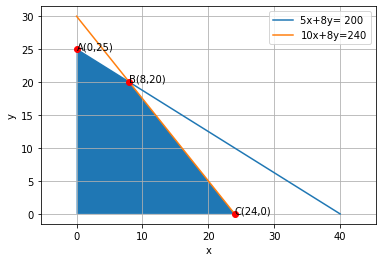
\includegraphics[width=\columnwidth]{solutions/su2021/2/18/Diagram.png}
\caption{Plywood Problem}
\label{fig:Plywood problem}	
\end{figure}

